\chapter{Problem Domain and Technological Base Concepts} \label{chap:sota}

\section*{}

%\begin{Notes}
%- Change transcriptome assembly to read alignment.\\
%\end{Notes}

In this chapter we begin by making a more in-depth presentation of the process
of gene expression. This will be followed by a literature and state-of-the-art
review in the fields of read alignment, differential expression analysis and
data mining. We will present the tools used in the development of the analysis
pipelines and the web platform. Lastly, we review some results evaluation
techniques and relevant data representation formats for genetic information.

\section{Biological Base Concepts}

%\begin{Notes}
%- Base concepts look good.\\
%- Include part about RNA binding proteins.\\
%\end{Notes}

Before dwelling in the details of the state of the art that are on the
foundation of the thesis, it is important to explain some concepts of the
domain of molecular biology.

\subsection{Gene Expression}

As explained in Chapter \ref{chap:intro}, gene expression is the mechanism by
which an organism's \dna{} can be expressed into functional genetic products,
like proteins. This process starts with the genetic code, or nucleotide
sequence, of each gene. Different genes in an organism's \dna{} are responsible
for the creation of different genetic products. The process of gene expression
itself is composed by two main stages, transcription and translation
\cite{leic:gene_expr}.

Transcription is the stage at which genetic data in the form of \dna{} is used
to synthesize \rna{}, being this the process that concerns the thesis' main
question. Several different types of \rna{} are produced by this process,
including \emph{mRNA} (which specifies the sequences of amino acids that form a
protein), \emph{rRNA} and \emph{tRNA}, both later used in the translation stage. Simplifying
a gene's structure, it can be seen as composed by two types of sequences,
introns and exons, as seen in Figure \ref{fig:intron_exon}.

\begin{figure}[!htb]
  \begin{center}
    \leavevmode
    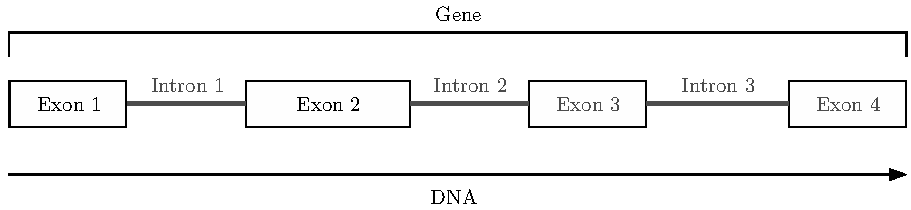
\includegraphics[width=1.0\textwidth]{intron_exon2}
    \caption[Overall structure of a gene]{Overall structure of a gene, with its
    different areas (simplified).}
    \label{fig:intron_exon}
  \end{center}
\end{figure}

The exons are useful in the gene expression process, being also known as coding
regions. Introns, on the other hand, are not used in the process. They are
present in an early stage mRNA molecule, the precursor mRNA, but are later
removed (or spliced) in the final molecule before the translation stage
\cite{leic:gene_expr}. Figure \ref{fig:splicing} illustrates the removal of
introns from the mRNA molecule, during the  splicing process.

\begin{figure}[!htb]
  \begin{center}
    \leavevmode
    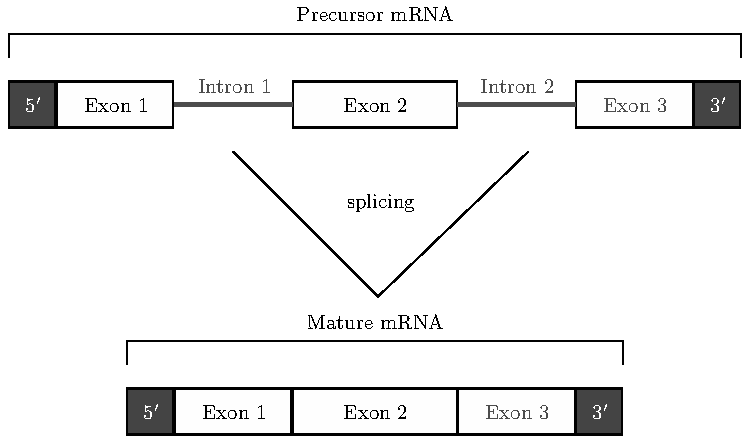
\includegraphics{splicing2}
    \caption[Removal of introns from precursor mRNA]{The removal (splicing) of
    introns from the precursor mRNA, during the transcription process.}
    \label{fig:splicing}
  \end{center}
\end{figure}

After the conclusion of the transcription process comes the translation process.
In this process, the synthesized mRNA is used to specify the sequence of amino
acids that constitute the particular protein being produced. The other types of
RNA molecules (rRNA and tRNA) are also used in this stage of the gene expression
process.

\subsection{RNA-Binding Proteins}

RNA-binding proteins, also referred to as RBP, regulate every aspect of the RNA
metabolism, including pre-mRNA splicing, mRNA transport, location, stability and
translation control \cite{Cooper2009777, Muller-McNicoll2013, Sonenberg2007721,
Sonenberg2009731}, as shown in Figure \ref{fig:rbp}.

\begin{figure}[!htb]
  \begin{center}
    \leavevmode
    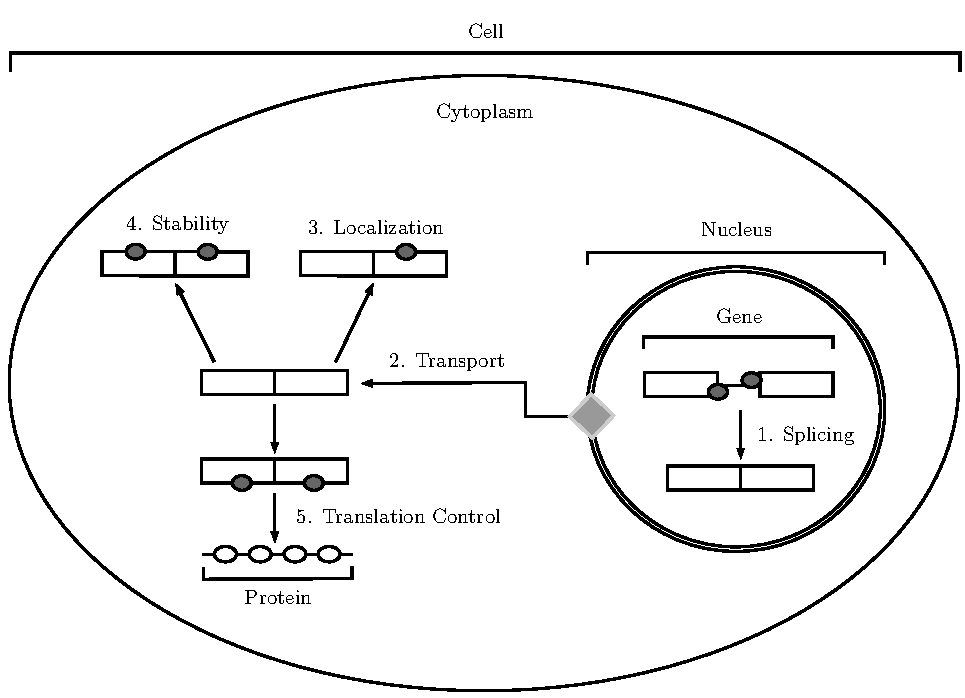
\includegraphics[width=\textwidth]{rbp}
    \caption[Role of RBPs in the RNA metabolism process]{
      Diagram of a typical cell showing the multiple roles of RBPs in post
      transcriptional processes \cite{janga2011construction}. The grey ellipses
      represent RBPs. The numbered text represents the different processes in
      which RBPs take part. Multiple RBPs can bind with a single RNA at one or
      more locations, creating an abundance of different combinations and
      possibilities in every step of the RNA metabolism.
    }
    \label{fig:rbp}
  \end{center}
\end{figure}

The binding of RBPs to RNA depends on different RNA-sequence specificities and
affinities. This aspect, coupled with the existence of hundreds of RBPs in an
organism, gives rise to a plethora of different combinations and outcomes to the
RNA metabolism.

RBPs regulate gene expression in health and disease, and mutations affecting the
function of RBPs may cause several diseases \cite{Cooper2009777}. Therefore,
understanding the binding patterns of RBPs during a particular biological
process is crucial to get insight into that process, both during health and
disease conditions.

\subsection{Sequencing}

Obtaining genetic information is done experimentally, by employing a sequencing
technique. For quite some time this process was carried out using the Sanger's
and other similar sequencing methods \cite{Reis-Filho2009}. Though
effective, such methods were notably slow and costly, with large projects like
the Human Genome Project (HGP) consuming roughly thirteen years and US\$ 3
billion. These limitations were so severe that, other than the realm of human
genetics, this kind of study was restricted to model organisms, such as the
fruit fly and mouse genomes \cite{Wolf2013}. The past few years have seen the
appearance and rise in popularity of the \ngs{} techniques. These techniques
differ from the more classical ones by producing larger amounts of information,
at lower cost. They are also typically more cost effective than previous
techniques and can be easily employed by single laboratories, which has greatly
contributed to their popularity.

The rise in popularity and availability of \ngs{} techniques, coupled with the
importance of RNA knowledge in understanding gene expression, led to the
appearance of RNA-Seq. RNA-Seq makes use of these newly available
deep-sequencing techniques to profile complete transcriptomes. This is, however,
a difficult task to accomplish. \ngs{} techniques produce shorter reads than
their older counterparts, being that \qt{\textit{(...) transcriptome assembly
from billions of RNA-Seq reads (...) poses a significant informatics challenge}}
\cite[p. 671]{Martin2011}.

Although this thesis does not deal with the problems of sequencing techniques, it
is important to indicate that the read data sets that were used resulted from
\ngs{} techniques, in particular RNA-Seq. As such, suitable tools for this
particular type of data were used.

\subsection{\Trans{} Assembly}\label{sec:transassembly}

%\begin{Notes}
%- Check microarrays sentence.\\
%\end{Notes}

\Trans{} assembly is the process by which experimentally obtained RNA data reads
can be organized and merged together in a partial or complete \trans. As stated
above, the advent of next generation sequencing techniques, with their reduced
costs, greatly increased the availability of transcript sequencing data.

For years, microarrays were the standard tool available for examining features
of the transcriptome and global patterns of gene expression \cite{Wolf2013}.
However, microarrays are typically more oriented towards assembly against
existing reference data, hence limiting its application to species with well
known reference genomes. This is a severe constraint, as \ngs{} techniques allow
to cheaply obtain genetic information of previously non-studied species. This is
one of the reasons that led to the inception of RNA-Seq. Contrary to
microarrays, RNA-Seq techniques are able to wield results that are suitable for
both reference guided assembly and \textit{de novo} assembly approaches
\cite{Wilhelm2009}. \textit{De novo} or exploratory assembly has captured the
interest of researchers in the past few years, leading to the appearance of
multiple RNA-Seq tools that are capable of making this type of assembly without
a reference genome \cite{nuno11:assemblathon}. Transcriptome assembly was not
performed during this thesis, as its main focus in terms of the RNA-Seq process
is read alignment and differential expression analysis.

\subsection{Relevant Standard File Formats}\label{sec:formats}

%\begin{Notes}
%- Describe the types of data present in each file type.\\
%\end{Notes}

As expected, the great diversity of RNA-Seq tools brings with it a wealth of
file formats. Some of these formats are developed from the ground up to satisfy
a specific need, while others are mere contextual adaptations or specializations
of already established formats. Below we will present a few of the most popular
and widely spread file formats, talking about their basic structure, the types
of data they represent and their applications. Some examples of this file
formats can be consulted in Appendix \ref{annex:formats}.

\subsubsection*{FASTA}

FASTA is the standard line and character sequence format used by NCBI
\cite{ncbi:fasta}, using this last organization's character code conventions
(see Appendix \ref{annex:fasta}). It is a simple format, that can be used to
easily store data represented by character sequences, like nucleotide (\dna,
\rna) or amino acid (protein) sequences. This file format is widely use to store
sequencing reads, \dna/\rna{} sequences and other character sequences in
database systems. Its simplicity makes it extremely easy to manipulate and
parse, presenting itself as an attractive solution for data transfer between
different tools.

\subsubsection*{FASTQ}

FASTQ is used to store character sequences, typically nucleotide sequences
\cite{Cock2010} (see Appendix \ref{annex:fastq}). It is quite similar to the
standard FASTA format, in respect to the manner in which character sequences are
represented. However, for every sequence, there is a second sequence of equal
length, representing the quality scores of the original sequence. These quality
scores are also represented as single characters, taking values between and
including ASCII-33 to ASCII-126. It is typically used in the same situations as
the FASTA format, when quality scores are available/relevant.

\subsubsection*{SAM and BAM}

The SAM format is a text format for storing sequence alignment data
\cite{genome:sam} (see Appendix \ref{annex:sam}). It is widely used to store
mapping information between sequencing reads and a given reference genome. This
sort of information is typically the product of sequencing alignment tools, that
consume sequencing reads from FASTQ files and align them with a reference
genome.

The BAM format contains exactly the same information as the SAM format and the
same rules apply for both formats. The difference between both formats lies in
their encoding. While SAM is a text based format, BAM is a binary format. This
means that BAM sacrifices human readability for increased machine processing
performance, as it is more efficient to work with compressed and indexed binary
data.

\subsubsection*{VCF}

VCF is a text file format used to store gene sequence variants \cite{smith13}
(see Appendix \ref{annex:vcf}). In the past few years, as larger and larger
genome sequencing projects became more common (like the 1000 Genomes
Project\footnote{The 1000 Genomes Project, started back in 2008, is an
international effort to establish the most comprehensive catalogue to date of
human genetic variations.}), storing such large amounts of information became a
serious concern. To address these concerns the VCF format was created. Instead
of storing the complete genome, VCF stores only the variations (and their
respective positions) of newly sequenced genomes relatively to a known reference
genome, typically in a compressed text file. As such, it is a format often used
when building genome databases.

\subsubsection*{GFF and GTF}

GFF is a text based file format to store gene features \cite{sanger11} (see
Appendix \ref{annex:gff}). Many genome assembly tools execute this process in
two separate steps: feature detection for identification of specific regions
(exons, introns, etc.) and genome assembly, using those features as reference.
However, it is beneficial to decouple these two steps, using different and more
efficient tools for each. As such, the GFF format emerged as a protocol for
feature information transfer between tools.

The GTF format is similar to the GFF format, in which it is based. It is also
used in similar situations. However, GTF builds on top of GFF, defining
additional conventions, specific to the domain of genetic information. Despite
their initial relation, both formats continue to be developed individually.

\section{RNA-Seq Analysis}

%\begin{Notes}
%- Describe the same workflow as iRAP.\\
%- Refer that we'll talk about specific tools below, and they all are Unix
%command line tools.
%\end{Notes}

\subsection{RNA-Seq Pipeline}

The analysis of RNA-Seq data is a complex process, with multiple stages. As
such, in order to produce relevant results is usually used a pipeline. An
analysis pipeline uses a set of tools, chained together in such a way that the
output of one tool becomes the input to the succeeding tool.

A typical RNA-Seq analysis pipeline is composed by six essential stages
\cite{rnaseqpipeline} (see Figure \ref{fig:rnaseq}):

\begin{description}

  \item[Read quality control and improvement]
  is a pre-processing stage. It comprises the usage of quality control tools,
  whose function is to trim bad quality data, in order to improve the overall
  quality of the data set. Other than direct data manipulation, this stage might
  produce some statistical data about the reads, that can later be used to
  better drive the succeeding stages.

  \item[Sample contamination checking]
  is also a pre-processing stage. As read data is obtained experimentally, it is
  not uncommon for contamination of the samples to occur. Bacterial
  contaminations, such as \emph{E. coli}, are fairly common and can sometimes
  skew the analysis results. In some cases it is possible to detect these
  contaminations and remove the affected data, hopefully improving the final
  results.

  \item[Read alignment]
  is the stage in which reads are positioned against a reference sequence. This
  sequence can be either a known and annotated reference genome (typically a
  combination of a FASTA file and a GTF file) or an assembled transcriptome,
  either assembled \emph{de novo} or against a reference genome (see Section
  \ref{sec:transassembly}). This alignment will allow to assess gene abundance
  in later stages of the pipeline.

  \item[Quantification]
  is the stage where transcript abundance is determined/estimated (gene
  expression). This involves counting the number of occurrences of certain
  transcripts in the read data. Typically this stage produces transcript count
  tables, that can later be used for differential expression analysis.

  \item[Differential expression]
  is the stage where transcript abundances between different samples are
  compared. As such, the produced count data is used to predict differences
  between transcript abundances between two or more samples, effectively
  demonstrating differences in gene expression. A common task for differential
  expression analysis is the comparison between a control and a mutated sample.

  \item[Result reporting]
  is the final stage in most pipelines. In this stage the resulting data is
  organized and represented in a manner that is useful to the user. This usually
  involves producing plots, tables and reports. Some pipelines may perform
  additional task before or after this stage, like gene set enrichment.

\end{description}

Note that this is only a generic architecture of a RNA-Seq analysis pipeline. In
practice new stages can be added and other can be removed, to better suit the
experiment at hand and the available data. In the given example (Figure
\ref{fig:rnaseq}) there is an additional stage, \emph{gene model parsing}, that
is only applied when the read are aligned against an annotated genome.

\begin{figure}[!htb]
  \begin{center}
    \leavevmode
    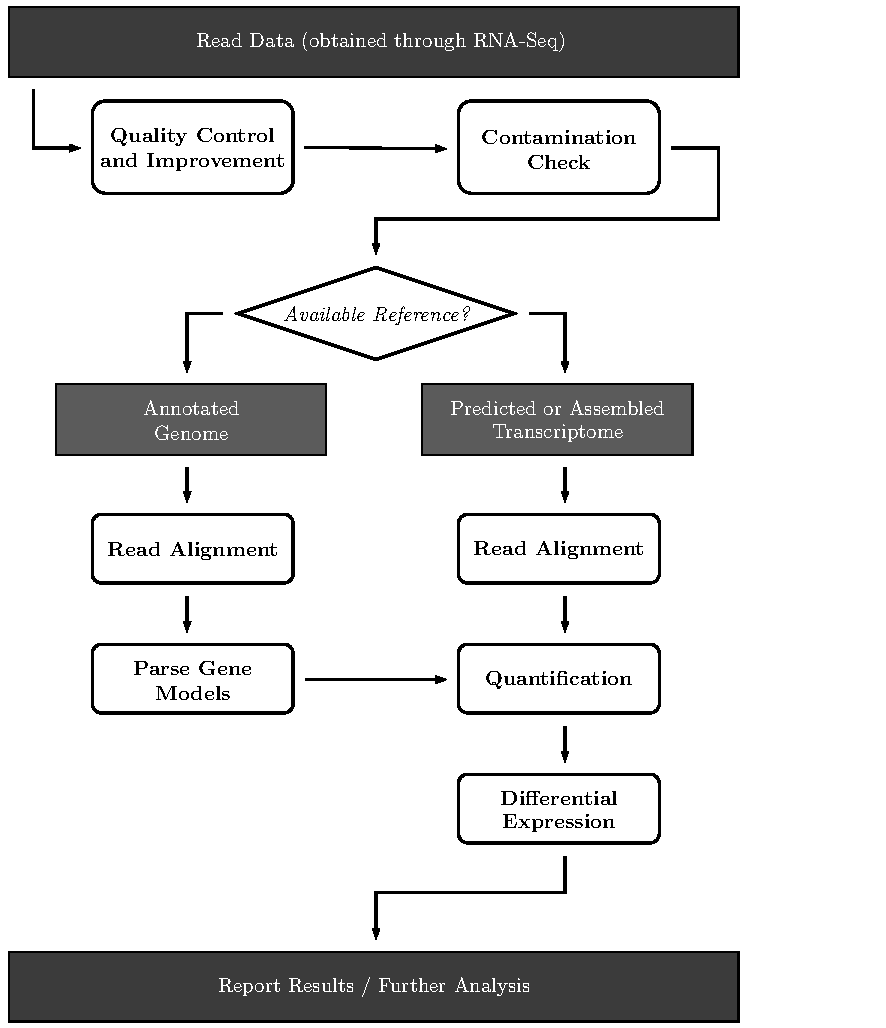
\includegraphics{rnaseq}
    \caption[Representation of a standard RNA-Seq analysis pipeline]{
      Representation of a standard RNA-Seq analysis pipeline
      \cite{rnaseqpipeline}. The analysis workflow has a slight variation
      depending on whether an annotated genome or an assembled transcriptome are
      used as reference for read alignment. Although this is a standard
      representation of the stages of RNA-Seq analysis, stages can be added or
      removed as needed to suit a particular assay.
    }
    \label{fig:rnaseq}
  \end{center}
\end{figure}

\subsubsection*{iRAP}\label{sec:irap}

iRAP\footnote{\url{https://code.google.com/p/irap/}} is a RNA-Seq analysis
pipeline \cite{irap}. It implements a workflow similar to the one described
above, albeit with some differences (see Figure \ref{fig:irap}). iRAP also
allows some stages of the analysis to be skipped. Differential expression
analysis is one such stage. This particular analysis will only be performed at
user request. The gene set enrichment stage (Figure \ref{fig:irap}, in dashed
line) is also optional. This stage uses Piano \cite{varemo01042013}, an R
package capable of conducting gene set analysis using various statistical
methods, from different gene level statistics and a wide range of gene-set
collections. However, this stage will not be analysed in-depth, as gene set
enrichment was not performed in this thesis.

One of the major strengths of iRAP is the ability to choose the tools that are
used in each stage \cite{irap}. This allows for a vast array of pipeline customization
possibilities, making it easy to adapt to a particular experiment. Below we will
present a set of tools, integrated in iRAP, that were used during this thesis.

iRAP requires is a minimum set of user provided information to perform RNA-Seq
analysis: the \emph{annotated reference genome} and the \emph{raw reads}, as
previously mentioned. Note that the reads are organized in libraries. A library,
in this case a cDNA library, is a collection of cDNA fragments that together
constitute a portion of the transcriptome.

\begin{figure}[!htb]
  \begin{center}
    \leavevmode
    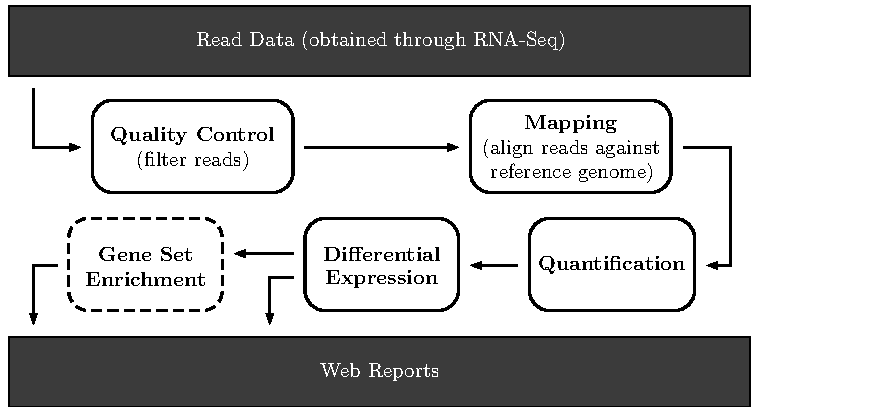
\includegraphics{irap}
    \caption[iRAP RNA-Seq data analysis pipeline]{
      iRAP RNA-Seq data analysis pipeline. Note that the gene enrichment step
      (in dashed line) is optional and was not used.
    }
    \label{fig:irap}
  \end{center}
\end{figure}

\subsection{\rnaseq{}, Read Alignment and Analysis Tools}\label{sec:seqtools}

We now present some bioinformatic tools, used to support the multiple steps of
the \rnaseq{}, read alignment and data analysis process. It is important to note
that none of these tools were used separately, but rather as parts of an
analysis pipeline (also described below).

\subsubsection*{Tuxedo Suite}

The Tuxedo suite is a free, open-source collection of applications that has been
widely adopted as analysis toolset for fast alignment of short reads. It is
composed by four separate tools (Bowtie, TopHat, Cufflinks and CummRbund)
briefly reviewed below. These tools are extensively used for \rnaseq{} analysis.
Although the applications are made for command line execution, there are several
workflow managers, like Galaxy\footnote{\url{http://galaxyproject.org/}}, that
easily integrates with the suite, providing a web interface for its use. Note
that not all components of the Tuxedo Suite were used.

\paragraph{Bowtie}

Bowtie is an ultrafast, memory-efficient short read aligner
\cite{langmead2009ultrafast}. Bowtie is typically used to build a reference
index for the genome of the organism being studied, for posterior use by other
tools, like TopHat. It can also output alignments in the standard SAM format,
allowing Bowtie to interoperate with tools like SAM Tools. However, it should
not be used as a general purpose alignment tool, as it was created and is more
effective when aligning short read sequences against large reference genomes.

\paragraph{TopHat}

TopHat is a fast splice junction mapper for \rnaseq{} reads
\cite{Trapnell01052009}. It uses Bowtie as the underlying alignment tool, using
its results and a FASTA formated reference genome to identify splice junctions
between exons.

\paragraph{Cufflinks}

Cufflinks assembles transcripts, estimates their abundances, and tests for
differential expression and regulation in \rnaseq{} samples
\cite{trapnell2010transcript}. It uses the SAM or BAM formatted files as input,
typically the ones produced by TopHat, outputting GTF files as a result.

\paragraph{CummeRbund}

Lastly, CummeRbund\footnote{\url{http://compbio.mit.edu/cummeRbund/}} is an R
package (see Section \ref{sec:clustertool}) designed to help the visualization and
analysis of Cufflinks' \rnaseq{} output. As such, it is not directly involved in
the trascriptome alignment process. It takes the various output files from
Cufflinks and uses them to build a SQLite database describing appropriate
relationships between genes, transcripts, etc. This database is later used to
convert that data to R objects which allows them to be used by plotting
functions, as well as by other commonly used data visualization tools.

\subsubsection*{HTSeq}

HTSeq is a programming framework used for processing data resulting from next
generation sequencing methods \cite{htseq}, developed in Python. While many
tools can efficiently align reads, sometimes data needs to be manipulated before
being passed to those tools. This data can either be badly formated (or
\qt{dirty}), or simply in a format different from the one that is needed. The
latter is a particularly common problem when trying to pass the results of one
tool to the one that succeeds it in the pipeline. HTSeq is useful to easily
create scripts that accomplish this task, acting as a \qt{glue} between tools.

HTSeq provides parsers for many popular formats for representing genetic
information (see Section \ref{sec:formats}). In addition, it ships with two
standalone scripts, HTSeq-QA and HTSeq-Count. HTSeq-QA is used to provide an
initial assessment of the quality of sequencing runs, producing plots with that
information. HTSeq-Count takes a SAM/BAM file and GTF/GFF file containing gene
models. It then counts, for each gene, how many aligned reads overlap that
gene's exons.

\subsection{Differential Expression Analysis Tools}

Below we describe the tools that were used for differential expression analysis.
These tools are integrated in the iRAP pipeline, are used in its fourth stage.

\subsubsection*{DESeq}

DESeq \cite{20979621} is available in an R package (see Section
\ref{sec:clustertool}), included in the Bioconductor super package. DESeq takes
count data generated from RNA-Seq analysis assays. As count data is discrete and
skewed, it is not well approximated by a normal distribution. DESeq solves this
problem by applying a test based on the negative binomial distribution, which
can reflect these properties. This method has a much higher power to detect
differential expression.

\subsubsection*{edgeR}

edgeR \cite{robinson2010edger} is available in an R package (see Section
\ref{sec:clustertool}), included in the Bioconductor super package. It provides
methods for the statistical analysis of count data from comparative experiments
on next generation sequencing platforms, among which is RNA-Seq, the most common
source of data used with edgeR. It has many characteristics in common with the
previously mentioned DESeq, as it also uses negative binomial models (among
others) to distinguish biological from technical variation. Later we describe
how both tools can be used together to produce better results.

\subsection{File Manipulation and Pre-processing Tools}

Sometimes data is badly formated or otherwise in a format that is not compatible
with a specific tool. This is particularly frequent when passing data between
two different tools in a pipeline. As such, we need some intermediate tools that
are able to easily manipulate and transform data, making it useful again. Below
we present some tools that can be used to accomplish this task.

\subsubsection*{SAM Tools}

SAM Tools\footnote{\url{http://samtools.sourceforge.net/}} is a library
package designed for parsing and manipulating alignment files in the SAM/BAM
format \cite{Li2009} (see Section \ref{sec:formats}). SAM Tools has two separate
implementations, one in C and the other in Java, with slightly different
functionality. Beyond manipulation of SAM and BAM files, this package is able to
convert between other read alignment formats, sort and merge alignments and show
them in a text-based viewer.

\subsubsection*{FASTX}

FASTX\footnote{\url{http://hannonlab.cshl.edu/fastx_toolkit/}} (FASTX-Toolkit)
is a collection of command line tools for pre-processing short read files. These
short read files can be either in FASTA or FASTQ format. FASTX is used to
manipulate these files before the aligning stage, in order to produce better
results. It includes tools to convert files from FASTQ to FASTA format, assess
statistics about the reads, filter and remove sequences based on their quality,
among others. Although the toolkit contains only command line based tools, some
of them are already integrated in the Galaxy web based workflow manager.

\subsubsection*{FastQC}

FastQC\footnote{\url{http://www.bioinformatics.babraham.ac.uk/projects/fastqc/}}
is a tool for quality control for \ngs{} data, implemented in Java. Its main
objective is to find errors and problematic areas in \ngs{} read data. FastQC
accepts FASTQ, SAM and BAM files, and is able to report results both inside the
tool itself and by exporting HTML files. These reports contain, among other
information, summary graphs and table that allow quick access to the data.
FastQC can either be used as a standalone tool with its graphical interface, or
as part of an analysis pipeline.

\section{Data Mining}\label{sec:mlearning}

%\begin{Notes}
%- Still relevant, don't change.\\
%- Important part is now clustering, not classification.
%\end{Notes}

Data mining is the process of \qt{\textit{extracting or \qt{mining} knowledge
from large amounts of data}} \cite[p. 5]{han2006data}. As such, it consists of a
set of techniques that can be used to find interesting patterns in large data
sets, that translate in newfound knowledge. Data mining borrows techniques from
multiple fields, such as artificial intelligence, machine learning, statistics,
and database systems \cite{Chakrabarti2012}. Its ultimate goal is to combine all
those techniques and transform large and (apparently) meaningless sets of data
into understandable and useful information. Thus, data mining was motivated by
the perspective of harnessing the abundance of data, that characterizes today's
information systems, to produce meaningful knowledge.

Because of their large quantities of input data, data mining tasks are usually
totally, or at least partially, automated. As such, there are several algorithms
for these tasks and tools that implement such algorithms, as presented in
Section \ref{sec:clusteralgo} and Section \ref{sec:clustertool}, respectively.

We can divide data mining into main types: \emph{descriptive data mining} and
\emph{predictive data mining} \cite{Fayyad1996}. Descriptive data mining is
focused on finding the underlying structure of a given set of data. Instead of
predicting future values, it concerns the intrinsic structure, relations and
interconnectedness of the data being analyzed, presenting its interesting
characteristics without having any predefined target. On the other hand,
predictive data mining is used to predict explicit values, based on patterns
determined from the data set. With predictive data mining we try to build models
using known data and use those models as a base to predict future behavior.

As we can see, data mining does not represent a single type problem. In fact
there are several different types of problems that can be addressed by data
mining techniques. Each of these problems may require a different data mining
method. A brief review of the most common type of problems is given below.

\begin{description}

  \item[Classification]
  is a type of problem that tries to generalize the already known structure of a
  data set, so that it applies to new data sets. In other words, with
  classification we try to learn a function that is capable of mapping our data
  into predefined classes.

  \item[Regression]
  tries to learn a function that models relationships between variables in the
  data set. That function can latter be used to find real value predictions of
  future behavior of data sets originated from the same population.

  \item[Clustering]
  consists in identifying a finite set of categories or clusters of similar
  values, to describe the data set. As such, it is used without prior knowledge
  about the data structure.

  \item[Summarization]
  provides a more compact representation of a subset of data, in a way that the
  summarized data retains the central points of the original data. This can be
  accomplished in several different ways, like using report generation or
  multivariate visualization techniques.

  \item[Dependency modeling]
  finds a model which describes relationships between variables, revealing their
  dependencies.

  \item[Change and deviation detection]
  tries to discover the most significant changes in the data, when compared with
  previously measured data. This method is useful to find interesting data
  variations or data errors.

\end{description}

Note that due to the nature of the work of this thesis we will focus on
clustering analysis techniques and, as such, the following sections will contain
a more in-depth review of these methods, along with descriptions of the used
algorithms and tools.

\subsection{Clustering Techniques}\label{sec:clustertech}

As explained above, clustering is the process of grouping data into
\emph{clusters}, in such a way that objects inside a cluster are very similar to
each other, while being as different as possible from objects in other clusters
\cite{han2006data}. These similarities (and dissimilarities) are assessed based
on the attributes of each object using a comparison method, often a distance
function. Clustering is used in situations where the classes contained in the
data set are unknown, either because they are difficult to determine or because
such an assessment would be too costly or we known little about the domain and
want to do a prospective study.

However, data clustering as a process is highly dependent on the data being
analysed. For example, while some data sets can be easily clustered using
\qt{spherical} clusters, other can only be represented by \qt{concave} clusters.
In other words, there is no global technique to group similar objects, it needs
to adapt to the problem at hand. This multitude of different interpretations of
the cluster notion led to the appearance of many different clustering methods
and algorithms. There are five major categories in which we can classify
clustering methods: \emph{partitioning methods}; \emph{hierarchical methods};
\emph{density-based methods}; \emph{grid-based methods}; and \emph{model-based
methods} \cite{han2006data}.

Generally, there are two major types of clustering methods, \emph{divisive
methods} and \emph{agglomerative methods}. In divisive methods all the objects
in the data set start in the same cluster. At each iteration all clusters are
divided into two smaller clusters, that better satisfy the fitness condition of
that particular algorithm. This process stops when all clusters are composed by
only one element. Inversely, agglomerative methods start with $n$ clusters with
one elements, joining them iteratively until only one cluster remains.

\subsubsection*{Partitioning Methods}

Partitioning methods are based around the construction of partitions of the
whole data set. Each one of the constructed partitions represents a data
cluster. Given a dataset with $n$ elements, and a number $k$ of clusters, the
correct application of these methods must verify two conditions
\cite{han2006data}:\\

\begin{tabular}{l l}
  (1) & each cluster must contain at least one object ($k \leq n$);\\
  (2) & a single object of the data set must only belong to one cluster.\\
\end{tabular}\\

These methods try to maximize cohesion between objects in the same partition,
while assuring that clusters are as distant as possible between themselves. In
other words, the elements within a partition should be as similar or \qt{close}
as possible between them, while being as different as possible from elements in
other groups.

Achieving the optimal partitioning would require the exhaustive enumeration and
combination of all possible clusters. This is, of course, impractical and even
unfeasible in some situations. As such, most partitioning methods adopt some
sort of heuristic evaluation of their clusters' quality. For example, the
\emph{k-means} algorithm uses the mean value of the objects in a cluster to
represent the same cluster; the \emph{k-medoids} algorithm, which is
centroid based, uses an object that is roughly at the center of the cluster to
represent it. Typically these methods work well with \qt{spherical} clusters,
but may falter with clusters having more complex shapes (\qt{concave} shaped
clusters, for example).

\subsubsection*{Hierarchical Methods}

These methods create an hierarchical division among objects in the data set.
This hierarchy is represented as a tree structure. There are two strategies for
hierarchical analysis, the \emph{divisive} strategy and the \emph{agglomerative}
strategy \cite{han2006data}. The \emph{divisive} strategy consists of putting
all objects in the same cluster and then divide them in multiple clusters, based
on their distance. This process is repeated iteratively, until every object is
in its own cluster. Inversely, the \emph{agglomerative} strategy starts by
putting each object in its own clustering, and then iteratively merges clusters
until all objects are part of one cluster.

One notable weak point of hierarchical methods is that calculated results are
irreversible; that is, once an objects is attributed to a cluster, that result
will not be evaluated again. This may lead to incorrect labeling of some
objects. These problems can be minimized by pre-processing the data set. Note
that this single pass evaluation gives hierarchical methods good computational
performance.

\subsubsection*{Density-based Methods}

Unlike the previous methods that rely on the notion of \emph{distance} between
objects, density-based methods are based on the notion of \emph{cluster density}
\cite{han2006data}. The basic idea of these methods is to keep growing a given
cluster while the number of objects in its vicinity (or \emph{density}) exceeds
a certain user defined threshold. Density-based methods are particularly useful
to discover clusters with irregular shapes. It should be noted that algorithms
implementing these kind of analysis, like DBSCAN \cite{Ester96adensity-based},
are usually very computationally heavy, both in terms of processing power and
memory usage
(although optimizations exist).

\subsubsection*{Grid-based Methods}

Grid-based methods transform the data set object space into a finite number of
cells, forming a grid structure
\cite{han2006data,DBLP:journals/corr/abs-1205-1117}. All clustering operations
are then conducted using the grid representation of the data set. Algorithms
that implement this strategy are usually high-performance, as execution times
are dependent on the number of cells in each dimension of the grid, rather than
on the number of objects in the data set.

\subsubsection*{Model-based Methods}

Model-based methods work by hypothesizing a mathematical model for each cluster
and then find the objects that best fit those models
\cite{DBLP:journals/corr/abs-1205-1117}. These methods typically follow the
assumption that objects are distributed by clusters according to an underlying
statistical probability. This also makes it possible for the number of clusters
to be automatically determined, based on such statistics \cite{han2006data}.

\subsection{Clustering Algorithms}\label{sec:clusteralgo}

Below we present the clustering algorithms that were used during the progress of
this thesis. These methods were chosen based on their suitability for the tasks
at hand, as will be described in Chapter \ref{chap:implementation}.

\subsubsection*{$k$-Medoids}

The $k$-medoids specification appeared as an evolution of the $k$-means
algorithm. As $k$-means uses the mean value of the objects of a cluster to
determine its center, it is sensitive to outliers (objects that deviate
considerably from the data set average): an object with a large, disproportional
value might skew the results. $k$-medoids mitigates this problem by using
medoids, picking a specific object of the cluster as its \qt{center}
\cite{han2006data}. Medoids are chosen randomly at the beginning. This means
that the algorithm may produce different results depending on the starting
objects (it does not reach an optimal solution). The remaining objects are then
clustered with the medoid to which they are most similar.

The most common implementation of $k$-medoids is the Partitioning Around
Medoids (PAM) algorithm (see Algorithm \ref{alg:pam}).

\begin{algorithm}
  \LinesNumbered
  \SetNlSty{texttt}{(}{)}
  \KwIn{$k$, the number of clusters; $D$, a data set containing $n$ objects.}
  \KwResult{A set of $k$ clusters.}
  \BlankLine

  \Repeat{no change}{
    assign each remaining object to the cluster with the nearest representative
    object\;
    randomly select a non-representative object, $o_{random}$\;
    compute the total cost, $S$, of swapping representative object, $o_{j}$,
    with $o_{random}$\;
    if $S < 0$ then swap $o_{j}$ with $o_{random}$ to form the new set of $k$
    representative objects\;
  }
  \BlankLine

  \caption[Partitioning Around Medoids (PAM) algorithm]{
    Partitioning Around Medoids (PAM) algorithm, a $k$-medoids implementation
    for partitioning based on medoid or central objects.
  }
  \label{alg:pam}
\end{algorithm}

\subsubsection*{Average Linkage Hierarchical Clustering}

Average linkage is a method for calculating distance between clusters in the
standard hierarchical clustering analysis. In order to decide which clusters
should be combined or divided, in agglomerative and divisive clustering
respectively, we need a measure of dissimilarity between those clusters. In the
average linkage method this dissimilarity is computed based on the average
distance between all elements in both clusters. The average is calculated over
all pairs of objects composed by one object from the first cluster and one
object from the second. The linkage function is therefore defined as
\begin{equation}
  \centering
  \label{eq:linkage}
  D(X, Y) = \frac{1}{N_{X} \times N_{Y}}\sum_{i=1}^{N_{X}}\sum_{j=1}^{N_{Y}}d(x_{i}, y_{i}), \quad x_{i} \in X, y_{j} \in Y 
\end{equation}
where $X$ and $Y$ are two clusters; $N_{X}$ and $N_{Y}$ and the number of
elements in clusters $X$ and $Y$, respectively; and $d(x_{i}, y_{j})$ is the
distance between objects $x \in X$ and $y \in Y$.

\subsubsection*{Inductive Logic Programming}

ILP is a subfield of machine learning that uses first order logic to represent
both data and models \cite{muggletonilp,Lavrac1998}. ILP infers hypotheses
(models) from examples and background knowledge. The examples may be of two
types: instances of the concept to be \qt{learned} (positive examples), and
non-instances of the concept (negative examples). Background knowledge is a set
of predicates encoding all information that the experts find useful to construct
the models. ILP might be used to tackle several machine learning and data mining
problems, like classification, regression, clustering and association rules
discovery.

The first and most important motivation for ILP systems is that they overcome
the representation limitations of attribute-value learning systems, such as the
previously mentioned data mining algorithms. Attribute-value systems base their
representations of data in table based representations. Although effective in
many situations, this representation is not very expressive and might not even
be feasible for certain problems \cite{Bratko:1995:AIL:219717.219771}. The
second motivation for ILP is that by using a logical representation, the
hypotheses are understandable and interpretable by humans, being therefore
useful to explain the phenomenons that produce the data. This representation
also means that background knowledge can be represented and employed in the
induction process, in contrast to attribute-value models, where this information
is difficult to represent. The expressive power of first-order logic enable an
easy representation of data with complex structure, and the encoding of complex
models that may combine numerical computation and relational information.

Despite these advantages, ILP cannot be applied indiscriminately to any
clustering or classification problems. ILP systems are typically very heavy when
it comes to computational resource consumption and run for long periods of time
\cite{fonseca2003implementation}. To ameliorate this situation there has been
significant progress in parallel execution of ILP systems.

\subsection{Clustering Evaluation and Assessment}\label{sec:clustereval}

The goal of most clustering methods is to achieve high similarity between
objects in the same cluster, while maintaining the dissimilarity between other
clusters \cite{Manning:2008:IIR:1394399}. This is called an \emph{internal
evaluation criterion}, as it is only dependent on the clustered data itself.
However, high internal evaluation scores do not necessarily translate to good
effectiveness in a real application.

To provide a better judgement of clustering results we may use \emph{external
criteria} \cite{Manning:2008:IIR:1394399}. Such criteria act as a surrogate for
the judgement of a human field expert. As such, they must use a set of data
outside the clustering data set, that was pre-classified by an expert. This set
of data is considered a \emph{golden standard}, that is, the best possible outcome for
the clustering analysis, under reasonable conditions.

Note that in the specific case of this thesis no pre-classified data set was
available. As such, we focused our assessments purely on internal evaluation
methods. Despite this lack of automated external evaluation, our results were
evaluated by experts in this field, as explained in Chapter \ref{chap:casestudy}.

\subsubsection*{Silhouette Coefficient}

The silhouette coefficient is a direct representation of the \emph{intra-cluster
similarity and inter-cluster dissimilarity} concept. In other words, the silhouette
coefficient improves as the cohesion between elements in the same group and the
farthest the distance from that particular group to all the other groups
\cite{Rousseeuw198753}. The silhouette coefficient is computed using the formula
\begin{equation}
  \centering
  \label{eq:silh}
  s(i) = \left\{\begin{array}{lcl}
  1 - \frac{a(i)}{b(i)}     & \quad \text{if}\ a(i) < b(i), \\
  0                         &  \quad \text{if}\ a(i) = b(i), \\
  \frac{b(i)}{a(i)} - 1     &  \quad \text{if}\ a(i) > b(i),
  \end{array}\right.
\end{equation}
where $a(i)$ is the average dissimilarity between $i$ and all other objects in
the same cluster; and $b(i)$ is the lowest average dissimilarity between $i$ and
any other cluster to which $i$ does not belong. The higher the value of $s(i)$,
the more appropriately clustered the data point is. Inversely, low silhouette
values are the result of unfitting clustering. The average $s(i)$ of a single
cluster can be used to measure how tightly all its data points are grouped. The
average $s(i)$ over the entire data set can be used to measure how appropriately
the data has been clustered.

The silhouette coefficient can also be used to provide a visual representation
of the clustering results, as dendograms do for hierarchical clustering
analysis (Figure \ref{fig:sil}). This plot combines silhouettes widths for all
objects in the data set, the average silhouette width for each cluster, and the
silhouette of the complete data set.

\begin{figure}[!htb]
  \begin{center}
    \leavevmode
    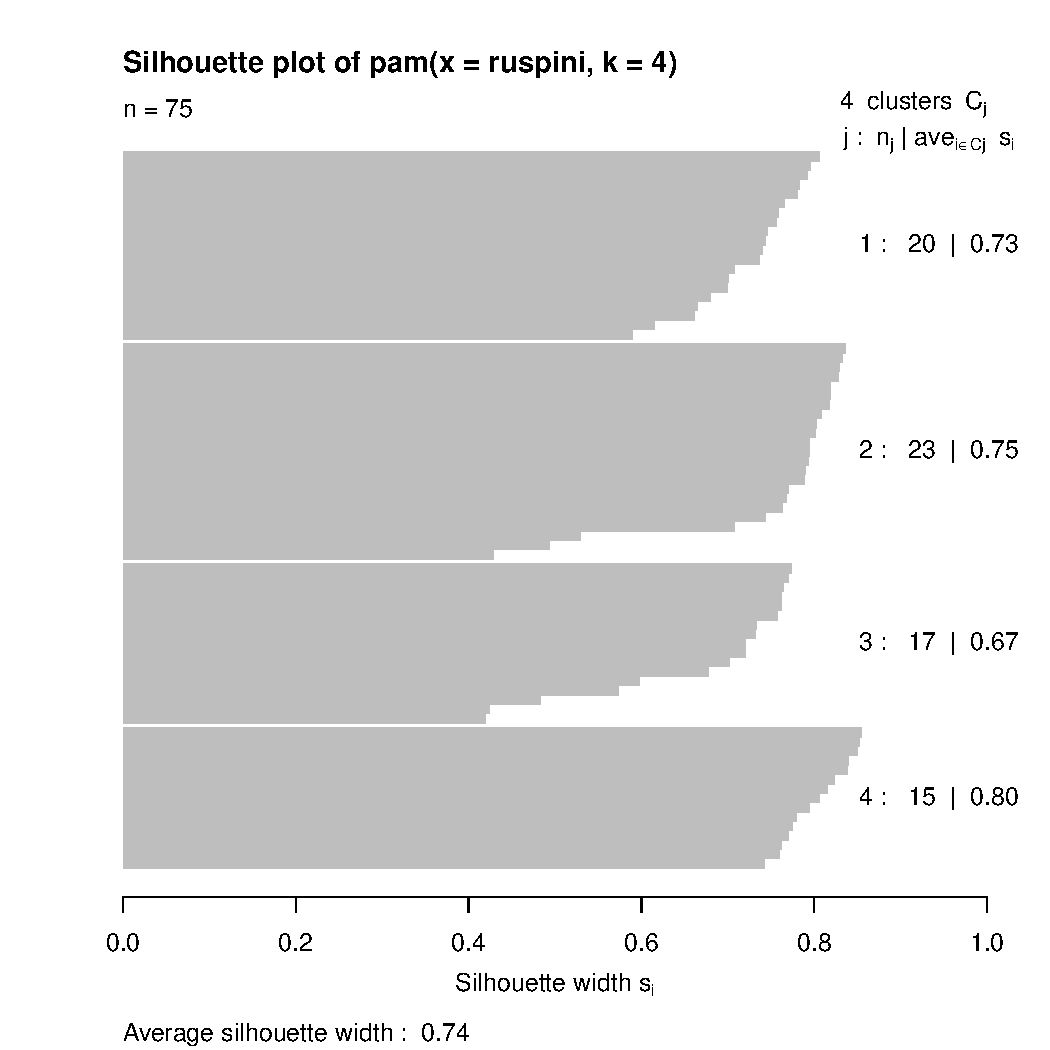
\includegraphics[width=0.9\textwidth]{sil}
    \caption[Example of a silhouette plot]{
      Example of a silhouette plot, using the PAM algorithm. It represents the
      silhouettes of every objects in the data set, as well as the average
      silhouette for each cluster ($k = 4$) and the average silhouette for the
      complete data set.
    }
    \label{fig:sil}
  \end{center}
\end{figure}

Other than that, the average silhouette of the clustering results may be used to
determine the best number of clusters. This is done by repeatedly executing the
analysis with different $k$ values, between a specified range. The chosen $k$
value is the one that produces the best average silhouette.

\subsection{Common Distance Measures}\label{sec:clusterdist}

Many clustering algorithms rely on the notion of \emph{distance} between objects
in the data set. These distances are used as a measure of
similarity/dissimilarity between those objects. Typically, objects that are
close to each other are considered similar, as opposed to objects that are far
away from each other and therefore considered different. Below we will present
some common types of distance measures that are used in clustering methods.

\subsubsection*{Euclidean Distance}

Euclidean distance is one the most common distance measures. It represents the
geometric distance between two points, in a $n$-dimensional space
\cite{DBLP:journals/corr/abs-1205-1117}. Euclidean distance can be defined as
shown in Equation \ref{eq:eucl} (for $n$-dimensions).
\begin{equation}
  \centering
  \label{eq:eucl}
  d(x, y) = \sqrt{\sum_{i = 1}^{n}\left | x_{i}  - y_{i}\right |^{2}}
\end{equation}

\paragraph{Squared Euclidean Distance}

The squared Euclidean distance is a simple variation of the stadard distance,
obtained by squaring it (Equation \ref{eq:sqeucl}). It is used when there is a
need to attribute progressively greater weight to objects that are far apart
from each other.
\begin{equation}
  \centering
  \label{eq:sqeucl}
  d(x, y) = \left (\sqrt{\sum_{i = 1}^{n}\left | x_{i}  - y_{i}\right |^{2}} \right)^{2} = \sum_{i = 1}^{n}\left | x_{i}  - y_{i}\right |^{2}
\end{equation}

\subsubsection*{Manhattan Distance}

The Manhattan distance between two objects is the sum of the differences between
each of their components. In other words, it is equivalent to the distance
between the two objects, if a $n$-dimensional grid-like path was followed
\cite{DBLP:journals/corr/abs-1205-1117}. It is defined as shown in Equation
\ref{eq:manhattan}.
\begin{equation}
  \centering
  \label{eq:manhattan}
  d(x, y) = \sum_{i = 1}^{n}\left | x_{i}  - y_{i}\right |
\end{equation}

\subsubsection*{Chebychev Distance}

The Chebychev distance is less common than the previously mentioned distances.
The Chebychev distance between two objects is defined as the maximum distance
between components of the objects (Equation \ref{eq:chev}). Is is useful in
situations where two object must necessarily be considered different if one of
their components is different, as the use of the maximum value removes the
dampening factors of other (closer) components.
\begin{equation}
  \centering
  \label{eq:chev}
  d(x, y) = max \left \{ \left | x_{i}  - y_{i} \right | \right \}
\end{equation}

\subsubsection*{Jaccard Distance}

The Jaccard distance is a measure of dissimilarity between two objects. It is
related to the Jaccard coefficient, a similarity measure. These measures are
applicable to binary and non-binary data. In these cases, a simple geometric
distance, like the Euclidean distance, might not accurately represent the
distance similarity (or dissimilarity) between the two objects.

For binary attributes, the Jaccard coefficient (similarity) is computed as
\begin{equation}
  \centering
  \label{eq:jacccoefbin}
  sim(x, y) = \frac{q}{q + r + s}
\end{equation}
where $q$ is the number of attributes that are true for both objects; $r$ is the
number of attributes that are true for object $x$ and false for object $y$; and
$s$ is the number of attributes that are false for object $x$ and true for
object $y$. Note that by definition the similarity coefficient is a value
between 0 and 1, where 0 indicates that the objects are completely different,
while 1 indicates that the objects are exactly equal. A distance measure can be
obtained directly from this coefficient, as shown in Equation
\ref{eq:jaccdistbin}.
\begin{equation}
  \centering
  \label{eq:jaccdistbin}
  dist(x, y) = 1 - sim(x, y)
\end{equation}
In this representation a value of 0 is given to two objects that are close,
while the value 1 is attributed to distant objects.

Similarly, the Jaccard coefficient and distance can be computed for sets. This
can be useful to determine distance between to objects whose attributes contain
nominal values. The Jaccard coefficient for sets is calculated as shown in
Equation \ref{eq:jacccoefset}, while the distance between sets is calculated in
the same way than between binary attributes.
\begin{equation}
  \centering
  \label{eq:jacccoefset}
  sim(x, y) = \frac{\left | x \cap y \right |}{\left | x \cup y \right |}
\end{equation}

\subsection{Clustering Tools}\label{sec:clustertool}

Except in rare cases of very specific problems, it typically makes no sense for
someone to implement any data mining algorithm that they might need. In fact,
today we have lots of data mining tools (many of which are free), that already
implement many of those algorithms. These tools are usually customizable, making
it easy to adapt them to most problems. Below we'll briefly review some of the
most popular data mining tools, applicable to the specific needs of this thesis.
Note that some of these tools, namely RapidMiner and Weka, were only used for
testing purposes during the development of the project. As such, they are not
part of the final prototype.

\subsubsection*{RapidMiner}

RapidMiner \cite{rapidminer} is a complete solution for data mining problems. it
is available as a standalone GUI based application, as seen in Figure
\ref{fig:rapidminer}. It is a commercial application, although its core and
earlier versions are distributed under an open source license and it offers a
free version, beyond its multiple paid versions. Being one of the most popular
data mining tools used today, its applications span several domains, including
education, training, industrial and personal applications, among others. Its
functionality can also be easily extended through the use of
plugins\footnote{Plugin is a software module that adds new functionality to an
existing software application. Plugins are typically dependent on the platform
they extend and can't be used as standalone tools.}, reflecting an increased
value for this tool. One of such example in the area of bioinformatics is the
integration plugin between RapidMiner and the
Taverna\footnote{\url{http://www.taverna.org.uk/}} open source workflow
management system \cite{Jupp2011}.

\begin{figure}[!htb]
  \begin{center}
    \leavevmode
    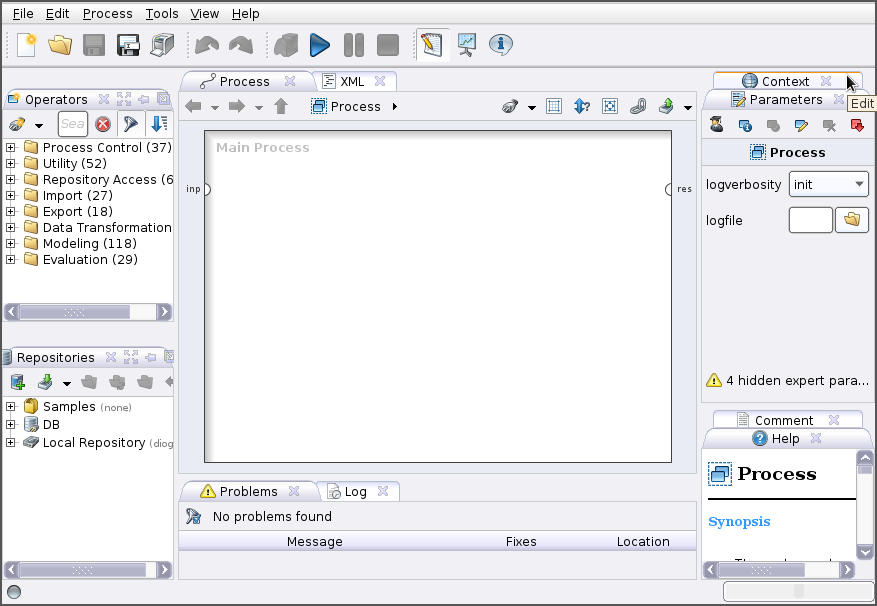
\includegraphics[width=1.0\textwidth]{rapidminer}
    \caption[RapidMiner user interface]{RapidMiner user interface.}
    \label{fig:rapidminer}
  \end{center}
\end{figure}

\subsubsection*{Weka}

Weka \cite{Hall} is an open source tool that implements several machine learning
algorithms and allows its user to easily apply those algorithms to data mining
tasks. Created at the University of Waikato, New Zeland in 1997\footnote{The
current version was completely rewritten in 1997, despite the first iteration of
the tool being developed as early as 1993.}, it is still in active development
to date. Weka supports several common data mining tasks, like data
preprocessing, classification, clustering, regression and data visualization.
Its core libraries are written in Java and allow for an easy integration of its
data mining algorithms in pre existing code and applications. Other than that,
Weka can be used directly through a command line/terminal or through one of its
multiple GUIs (Figure \ref{fig:weka}). Its simple API and well structure
architecture allow it to be easily extended by users, should they need new
functionalities.

\begin{figure}[!htb]
  \begin{center}
    \leavevmode
    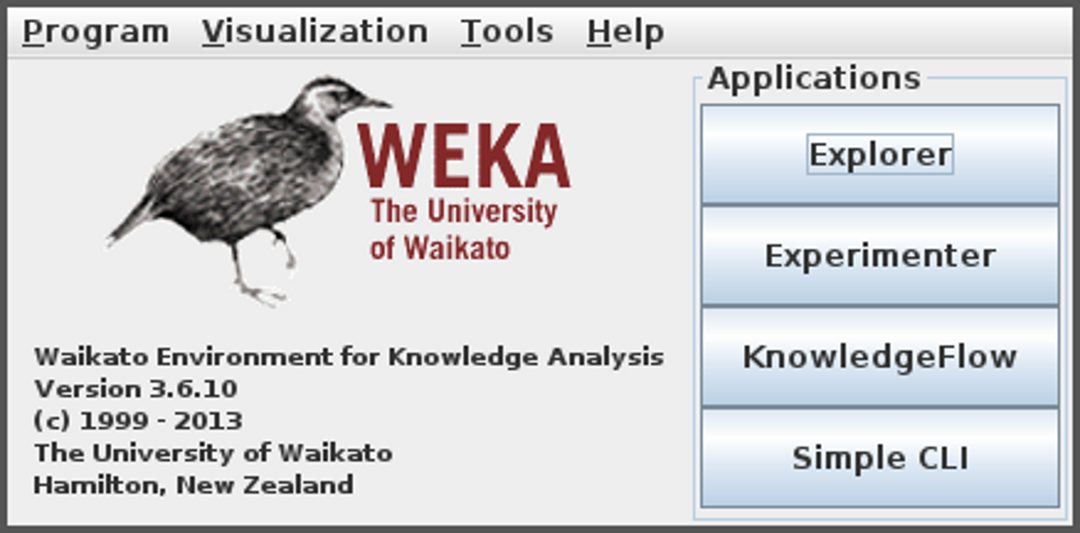
\includegraphics[width=0.7\textwidth]{weka}
    \caption[Weka interface selection]{Weka interface selection.}
    \label{fig:weka}
  \end{center}
\end{figure}

\subsubsection*{R Language}

R \cite{Ihaka1998} is a free programming language and software environment for
statistical computing and graphics generation. Originally developed by Ross
Ihaka and Robert Gentleman at the University of Auckland, New Zealand in 1993,
it is still under active development. R is typically used by statisticians and
data miners, either for direct data analysis or for developing new statistical
software \cite{Fox2005}.

R is an implementation of the S programming language\footnote{S is an object
oriented statistical programming language, appearing in 1976 at Bell
Laboratories.}, borrowing some characteristics from the Scheme programming
language. Its core is written in a combination of C, Fortran and R itself. It is
possible to directly manipulate R objects in languages like C, C++, Java and
Prolog. R can be used directly through the command line or through several third
party graphical user interfaces like
Deducer\footnote{\url{http://www.deducer.org/pmwiki/index.php}}. There are also
R wrappers for several scripting languages.

R provides several different statistical and graphical techniques, including
linear and nonlinear modeling, classical statistical tests, time-series
analysis, classification, clustering, among others. It can also be used to
produce publication-quality static graphics. Tools like Sweave
\cite{lmucs-papers:Leisch:2002} allow users to embed R code in \LaTeX{}
documents, for complete data analysis.

\paragraph{Bioconductor Package}

Bioconductor is a free and open source set of tools for genomic data analysis,
in the context of molecular biology \cite{lmucs-papers:Leisch:2002}. It is
primarily based on R. It is under active development, with two stable releases
each year. Counting with more than seven hundred different packages, it is the
most comprehensive set of genomic data analysis tools available for the R
programming language. It contains many of the tools that are part of most open
source biological analysis pipelines. It also provides a set of tools to read
and manipulate several of the most common file formats used in molecular biology
oriented applications, including FASTA, FASTQ, BAM and GFF.

\section{Chapter Conclusions}

In this chapter we gave a brief introduction of the molecular biology concepts
that serve as base of the thesis. We have reviewed the concepts on RNA-Seq and
data mining and presented short analyses of concrete tools and algorithms that
were used during this thesis.
